% Created 2024-11-12 周二 11:13
% Intended LaTeX compiler: xelatex
\documentclass[a4paper, 11pt]{article}
\usepackage{graphicx}
\usepackage{longtable}
\usepackage{wrapfig}
\usepackage{rotating}
\usepackage[normalem]{ulem}
\usepackage{capt-of}
\usepackage{hyperref}
\author{忻斌健}
\date{2023.01.12}
\title{BLMP深度学习方法总结}
\hypersetup{
 pdfauthor={忻斌健},
 pdftitle={BLMP深度学习方法总结},
 pdfkeywords={},
 pdfsubject={},
 pdfcreator={忻斌健}, 
 pdflang={English}}
\begin{document}

\maketitle
\setcounter{tocdepth}{1}
\tableofcontents

\section*{电池银行大数据模型}
\label{sec:org029afb7}
\subsection*{数据来源:}
\label{sec:orgc4bf967}
\begin{itemize}
\item 信号:单体电芯电压
\item 场景:充电
\begin{itemize}
\item 函数: \(V\) ; 自变量:电压,电流,温度, \(SoC\), \(SoH\), \(SoS\), \ldots{}

\begin{align*}
    V &=f(I,T,SoC,SoH,SoS,...)\\
      &\approx\hat{f}(I,SoC,SoH,SoS,...)
\end{align*}
\end{itemize}

\item 函数求逆

\(SoS \approx \hat{f}^{-1}(V,I,SoC,SoH,...), SoS \in \{Good, Bad\}\)
\end{itemize}
\subsection*{随机模型}
\label{sec:org9e63245}

\begin{itemize}
\item 获得安全状态和观测量之间的关系:\(SoS \approx \hat{f}^{-1}(V,I,SoC,SoH,...), SoS \in \{Good, Bad\}\)
\end{itemize}
\begin{itemize}
\item 随机模型:
\begin{itemize}
\item 不能找到精确的关系
\begin{itemize}
\item 确定允许的误差
\item 缩小不确定性
\end{itemize}
\item 非确定性,概率判定
\item 可定量计算
\end{itemize}
\item 目标:
\begin{itemize}
\item 估计概率分布模型
\begin{itemize}
\item 规律性(regularity)
\item 观测量(时间特征)
\item 大数据
\end{itemize}
\end{itemize}
\end{itemize}
\subsection*{深度学习信号模型}
\label{sec:org6bf7bf2}
\begin{center}
\includegraphics[width=.9\linewidth]{c:/msys64/home/xinbinjian.sh/.org.d/roam/img/20230111_112316dl1.png}
\end{center}
\begin{center}
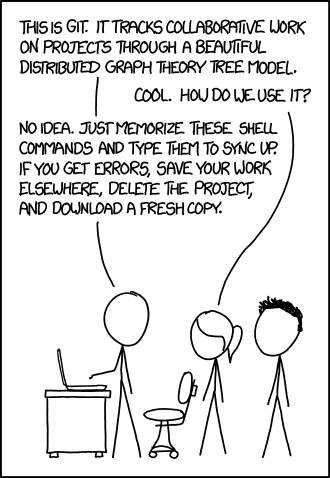
\includegraphics[width=.9\linewidth]{c:/msys64/home/xinbinjian.sh/.org.d/roam/img/20230111_112041dl2.png}
\end{center}
\begin{itemize}
\item 时间序列观测量 \(\mathcal{X}_t\): (\(U_t\), \(I_t\),\ldots{})
\begin{itemize}
\item 场景选择
\item 特征选择
\end{itemize}
\item 参数 \(\mathcal{S}\): (\(SoS\), \(SoC\), \(SoH\), \(T\),\ldots{})
\end{itemize}
\begin{itemize}
\item 压缩时间序列 \(\mathcal{H}_{\mathcal{X}_t}\)
\item 压缩隐藏参数  \(\mathcal{H_{\mathcal{s}}}\)
\item 鉴别器(隐空间 Discriminator)直接输出离群度作为定量判别依据
\end{itemize}
\subsection*{深度学习网络模型}
\label{sec:orgf85d30a}
可观测性假设:低维度信号(\(\mathcal{S}: (SoS, SoC, SoH,...)\)
决定高维度信号 \(\mathcal{X}_t: (U_t, I_t)\) 分布
\begin{figure}[htbp]
\centering
\includegraphics[width=.9\linewidth]{c:/msys64/home/xinbinjian.sh/.org.d/roam/img/20230111_122019dl3.png}
\caption{时间序列 GAN 模型}
\end{figure}


\begin{itemize}
\item 时间序列自动编解码器
\begin{itemize}
\item 压缩映射到隐空间
\item 降低维度提高效率
\end{itemize}
\item 监督学习
\begin{itemize}
\item 提高时间特性学习效率
\end{itemize}
\item 生成对抗网络(GAN)
\begin{itemize}
\item 隐空间训练
\item 掌握数据分布
\item 生成逼真的数据
\end{itemize}
\end{itemize}
\subsection*{深度学习特点}
\label{sec:org273131b}
\begin{itemize}
\item 无监督学习
\begin{itemize}
\item 学习数据分布
\item 经验知识的数学模型
\item 从大数据中提炼信息,规律,知识
\end{itemize}
\item 高效可持续消化大数据
\item 选择合适的特征可极大提高效率
\item 方法和模型的快速改善
\end{itemize}
\subsection*{机器学习运维模式(云服务器)MLOps}
\label{sec:orgd2e9b34}

\begin{center}
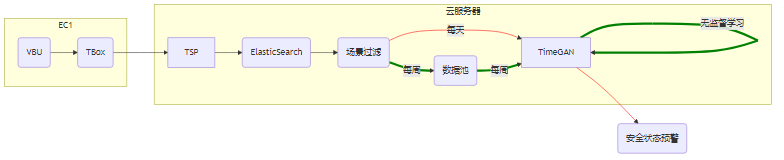
\includegraphics[width=.9\linewidth]{./img/funes-production.png}
\label{Fig. Dataflow}
\end{center}


\begin{figure}[htbp]
\centering
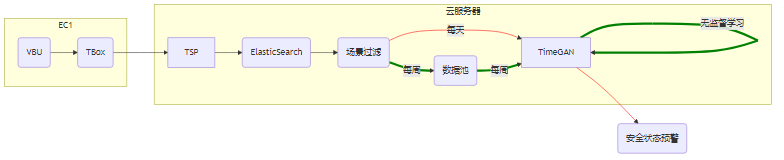
\includegraphics[width=.9\linewidth]{./img/funes-production.png}
\caption{\label{Fig. Dataflow}训练和推理的数据流}
\end{figure}
\section*{结果}
\label{sec:org22b4047}
\subsection*{无监督学习训练}
\label{sec:orge2e708c}
\subsubsection*{数据样本}
\label{sec:org7ee37eb}
数据分布由给定样本集合确定(训练集,验证集,测试集)
\begin{itemize}
\item 复杂度可控的模拟样本
\begin{itemize}
\item 正弦波:随机采样参数相位,频率,自由度 N=2
\item 三角波:随机采样参数相位,频率,斜率,自由度 N=3
\end{itemize}
\item 真实样本:
\begin{itemize}
\item 原始单体电压充电场景下时间序列,自由度 N=?
\begin{itemize}
\item 充电 80\%~100\%(充满)
\item 在多种形态下选择最常见的一种,肉眼判断约占总样本 20\%
\end{itemize}
\item 固定自由度的三次样条拟合原始单体电压
\begin{itemize}
\item 保持基本形态的前提下,降低复杂度
\item 选择位置固定的节点,保持基本形态,节点数 N=11
\item 随机采样节点横向和纵向扰动,自由度 3N
\end{itemize}
\end{itemize}
\end{itemize}
\subsubsection*{验证}
\label{sec:org0522e7e}
\begin{itemize}
\item 从冻结的生成器(Generator)随机采样
\item 从训练样本中匹配最相似时间序列
\item 压缩空间聚类可视化
\item 从不同样本集采样,交叉验证
\end{itemize}
\subsubsection*{正弦波的生成模型训练和采样结果(单模态)}
\label{sec:orgcc4d54d}
\begin{center}
\includesvg[width=.9\linewidth]{c:/msys64/home/xinbinjian.sh/.org.d/roam/img/_20230112_103534fft_most_similar_cases-20220920-095753}
\end{center}
\begin{center}
\includesvg[width=.9\linewidth]{c:/msys64/home/xinbinjian.sh/.org.d/roam/img/_20230112_101420fft_most_similar_cases-20220921-153548}
\end{center}
\begin{center}
\includesvg[width=.9\linewidth]{c:/msys64/home/xinbinjian.sh/.org.d/roam/img/_20230112_101501fft_most_similar_cases-20220921-152459}
\end{center}
\begin{center}
\includesvg[width=.9\linewidth]{c:/msys64/home/xinbinjian.sh/.org.d/roam/img/_20230112_102209fft_most_similar_cases-20221109-094318}
\end{center}
\subsubsection*{正弦波的压缩空间聚类(单模态)}
\label{sec:org9a239a6}
\begin{center}
\includesvg[width=.9\linewidth]{\detokenize{c:/msys64/home/xinbinjian.sh/.org.d/roam/img/无监督学习训练/_20230112_151750pca-20220921-090946}}
\end{center}

\begin{center}
\includesvg[width=.9\linewidth]{\detokenize{c:/msys64/home/xinbinjian.sh/.org.d/roam/img/无监督学习训练/_20230112_154535tsne-20220921-090953}}
\end{center}

\begin{center}
\includesvg[width=.9\linewidth]{\detokenize{c:/msys64/home/xinbinjian.sh/.org.d/roam/img/无监督学习训练/_20230112_155054pca-20221109-094252}}
\end{center}
\begin{center}
\includesvg[width=.9\linewidth]{\detokenize{c:/msys64/home/xinbinjian.sh/.org.d/roam/img/无监督学习训练/_20230112_155207tsne-20221109-094301}}
\end{center}
\subsubsection*{正弦波的模拟离群点检测(单模态)}
\label{sec:org4f6602d}
\begin{center}
\includesvg[width=.9\linewidth]{\detokenize{c:/msys64/home/xinbinjian.sh/.org.d/roam/img/无监督学习训练/_20230112_160536Data_Logits-20221109-094833}}
\end{center}

\begin{center}
\includesvg[width=.9\linewidth]{\detokenize{c:/msys64/home/xinbinjian.sh/.org.d/roam/img/无监督学习训练/_20230112_160746outlier_pca-20221109-094858}}
\end{center}
\begin{center}
\includesvg[width=.9\linewidth]{\detokenize{c:/msys64/home/xinbinjian.sh/.org.d/roam/img/无监督学习训练/_20230112_160657Data_Logits-20221109-095411}}
\end{center}
\begin{center}
\includesvg[width=.9\linewidth]{\detokenize{c:/msys64/home/xinbinjian.sh/.org.d/roam/img/无监督学习训练/_20230112_160848outlier_pca-20221109-095421}}
\end{center}
\subsubsection*{三角波的生成模型训练和采样结果(单模态)}
\label{sec:org9a9f017}
\begin{center}
\includesvg[width=.9\linewidth]{\detokenize{c:/msys64/home/xinbinjian.sh/.org.d/roam/img/无监督学习训练/_20230112_162940fft_most_similar_cases-20221109-131947}}
\end{center}
\begin{center}
\includesvg[width=.9\linewidth]{\detokenize{c:/msys64/home/xinbinjian.sh/.org.d/roam/img/无监督学习训练/_20230112_163112pca-20221109-131922}}
\end{center}
\begin{center}
\includesvg[width=.9\linewidth]{\detokenize{c:/msys64/home/xinbinjian.sh/.org.d/roam/img/无监督学习训练/_20230112_163412Data_Logits-20221109-132846}}
\end{center}
\begin{center}
\includesvg[width=.9\linewidth]{\detokenize{c:/msys64/home/xinbinjian.sh/.org.d/roam/img/无监督学习训练/_20230112_163625outlier_pca-20221109-132853}}
\end{center}
\subsubsection*{充电电压样条拟合数据的生成模型训练和采样结果}
\label{sec:org05d435e}
\begin{center}
\includesvg[width=.9\linewidth]{\detokenize{c:/msys64/home/xinbinjian.sh/.org.d/roam/img/无监督学习训练/_20230112_165616most_similar_cases-20221108-105611}}
\end{center}
\begin{center}
\includesvg[width=.9\linewidth]{\detokenize{c:/msys64/home/xinbinjian.sh/.org.d/roam/img/无监督学习训练/_20230112_165759pca-20221108-105544}}
\end{center}
\begin{center}
\includesvg[width=.9\linewidth]{\detokenize{c:/msys64/home/xinbinjian.sh/.org.d/roam/img/无监督学习训练/_20230112_170336Data_Logits-20221109-105440}}
\end{center}
\begin{center}
\includesvg[width=.9\linewidth]{\detokenize{c:/msys64/home/xinbinjian.sh/.org.d/roam/img/无监督学习训练/_20230112_170835outlier_pca-20221109-105448}}
\end{center}
\subsubsection*{混合时间序列(正弦与三角)生成模型和采样结果(多模态)}
\label{sec:org2e8aa1f}
\begin{center}
\includesvg[width=.9\linewidth]{\detokenize{c:/msys64/home/xinbinjian.sh/.org.d/roam/img/无监督学习训练/_20230112_172308fft_most_similar_cases-20221108-131528}}
\end{center}
\begin{center}
\includesvg[width=.9\linewidth]{\detokenize{c:/msys64/home/xinbinjian.sh/.org.d/roam/img/无监督学习训练/_20230112_172620pca-20221108-131502}}
\end{center}
\begin{center}
\includesvg[width=.9\linewidth]{\detokenize{c:/msys64/home/xinbinjian.sh/.org.d/roam/img/无监督学习训练/_20230112_174828outlier_pca-20221109-113016}}
\end{center}
\begin{center}
\includesvg[width=.9\linewidth]{\detokenize{c:/msys64/home/xinbinjian.sh/.org.d/roam/img/无监督学习训练/_20230112_174534outlier_tsne-20221109-113023}}
\end{center}
\subsection*{监督学习}
\label{sec:orga97b3a0}
\subsubsection*{可理解的时间序列特征,监督学习训练成熟稳定}
\label{sec:org5207179}
\begin{center}
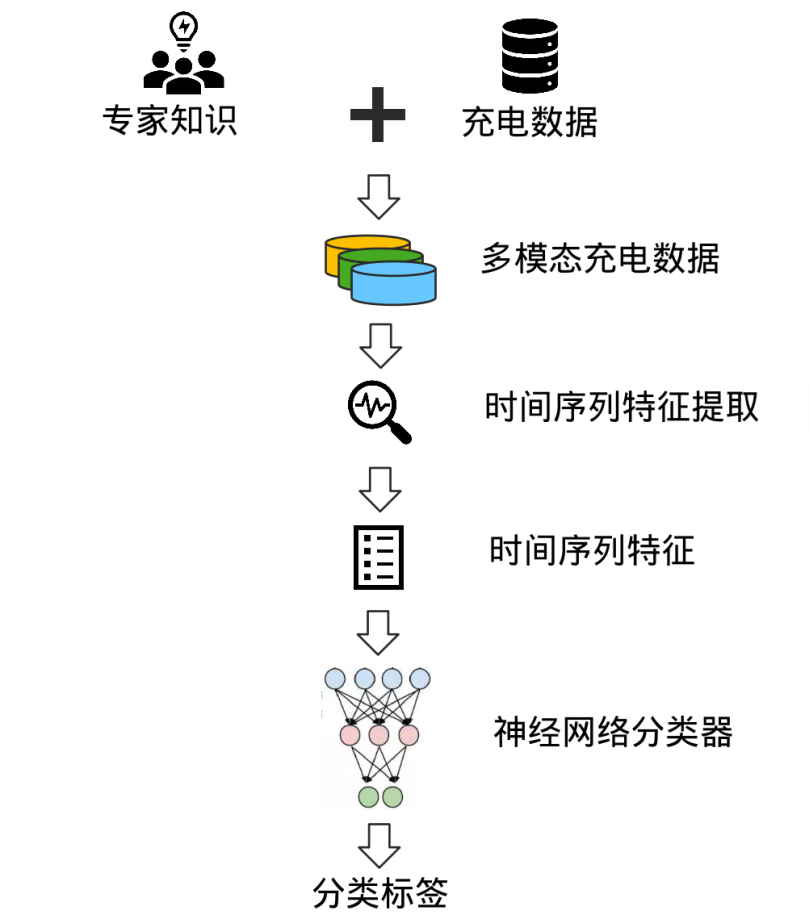
\includegraphics[width=.9\linewidth]{c:/msys64/home/xinbinjian.sh/.org.d/roam/img/监督学习/_20230112_180524ts_supervised_learning.png}
\end{center}
\begin{itemize}
\item 数据样本是已标注的多模态数据(含离群数据和多模态正常数据)
\item 利用时间序列通用特征 FAIR(KAT,65 个特征)
\begin{itemize}
\item 均值,方差,中值,过中线次数
\item 自相关,鲁棒性统计量,季节性变化系数,趋势系数
\item Hurst 指数(自相关系数随时间衰落的指数(長時记忆)),KPSS 测试(稳态表征)
\end{itemize}
\end{itemize}
\subsubsection*{监督学习的优点}
\label{sec:org4928129}
\begin{itemize}
\item 结果可解释,主要依据专家知识(标签,可解释特征)
\item 利用专家知识和时间序列特征区分不同模态
\item 可与专家交互,判断和定义新模态,迭代更新模型
\item 高效处理已知且特征可描述的异常数据,专家只需处理新的模态
\item 利用反向传播算法确定特征作用的权重,筛选相关特征
\end{itemize}
\subsubsection*{结果}
\label{sec:org55cd601}
\begin{center}
\includesvg[width=.9\linewidth]{\detokenize{c:/msys64/home/xinbinjian.sh/.org.d/roam/img/监督学习/_20230112_185237KATS_Data_Logits-20221109-173756}}
\end{center}
\begin{center}
\includesvg[width=.9\linewidth]{\detokenize{c:/msys64/home/xinbinjian.sh/.org.d/roam/img/监督学习/_20230112_185445KATS_Data_Logits-20221109-165456}}
\end{center}
\begin{center}
\includesvg[width=.9\linewidth]{\detokenize{c:/msys64/home/xinbinjian.sh/.org.d/roam/img/监督学习/_20230112_1856405_vol_PCA-20221111-155631}}
\end{center}
\begin{center}
\includesvg[width=.9\linewidth]{\detokenize{c:/msys64/home/xinbinjian.sh/.org.d/roam/img/监督学习/_20230112_1857055_vol_t-SNE-20221111-155637}}
\end{center}
\section*{总结(工具箱 )}
\label{sec:org505ddb1}
\begin{itemize}
\item 弱特征(原始数据): LSTM/GRU 形式的时间序列对抗生成网络
\begin{itemize}
\item 低复杂度信号的构造和快速闭环反馈调试
\item 以原始数据为目标的评估
\item 生产环境原始信号低复杂度拟合与训练
\item 需要明确单体电压充电工况的模态特征波形
\end{itemize}
\item 强特征:利用通用时间序列特征(KAT)的监督学习方法
\begin{itemize}
\item 专家在环的开发方式
\item 自动评估特征对分类的重要性权重
\end{itemize}
\item 估计信号复杂度以及和计算资源关系
\item 试运行生产环境的机器学习运维
\begin{itemize}
\item 训练: 每周场景数据自动收集,训练与模型更新
\item 推理:场景数据自动获取和推理报警
\end{itemize}
\end{itemize}
\subsection*{挑战}
\label{sec:orge6f60c0}
\subsubsection*{时间序列特征工程}
\label{sec:org66a3be2}
\begin{itemize}
\item 建模困难
\item 不像图像和自然语言,无法利用已有的人类知识,概念
\item 已有的经验知识表述不系统,不确定度高前后不一致
需要收集和分析经验知识
\end{itemize}
\subsubsection*{机器学习}
\label{sec:org80aee91}
\begin{itemize}
\item RNN 对长的时间序列数据(>100)较难训练
\item GAN 训练不稳定
\item 计算资源瓶颈
目前复杂度上限:隐藏维度 8,层数 2,batch 32
\item 训练样本不足
目前符合要求的时间序列<10000
\end{itemize}
\subsubsection*{时间序列模型构建}
\label{sec:org0d2f9ed}
\begin{itemize}
\item 场景选择影响信号的复杂度
\item 时间序列特征选择影响模型结构和超参选择
\item 独立于场景选择的通用模型,依赖条件模型的训练
增加输入时间序列信号的维度,极大增加复杂度
\end{itemize}
\subsection*{机遇}
\label{sec:orgc13237c}
\subsubsection*{经验知识和大数据结合}
\label{sec:orgc047620}
\begin{itemize}
\item 专家在环迭代
\begin{itemize}
\item 专家知识可被机器学习模型吸收
\item 减轻重复人工劳动
\end{itemize}
\item 深度学习是目前最好的大数据技术
\end{itemize}
\subsubsection*{模型改进}
\label{sec:orgbc2840b}
\begin{itemize}
\item Transformer 模型取代 GRU/LSTM
\item 条件推理模型
\item 多模态聚类隐空间改进
\item 基础模型作为服务(Model as Service)
\end{itemize}
\subsubsection*{扩散模型 diffusion model}
\label{sec:orgf1054ba}
\begin{itemize}
\item 稳定有效对数据分布进行变换的深度学习方法
\item 静态分布估计到概率函数分布变换
\item 计算资源,单机单卡可以进行推理
\item 效率提升:半年 1000x 加速
\item 跨领域应用:图像,自然语言,视频,音频
\end{itemize}
\subsubsection*{图像扩散模型用于补全}
\label{sec:org3f78272}
\begin{center}
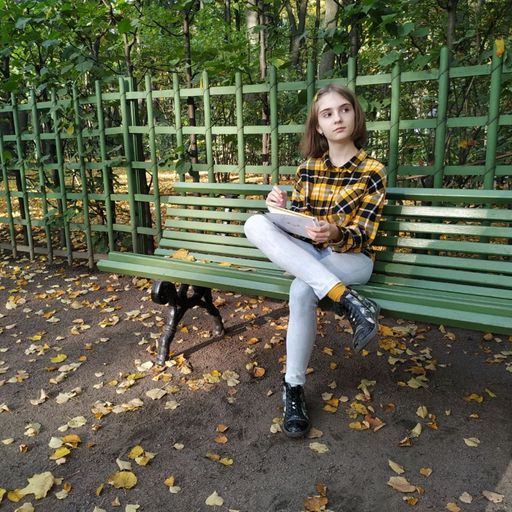
\includegraphics[width=.9\linewidth]{c:/msys64/home/xinbinjian.sh/.org.d/roam/img/扩散模型_diffusion_model/_20230112_192239bench2.png}
\end{center}
\begin{center}

\includegraphics[width=.9\linewidth]{c:/msys64/home/xinbinjian.sh/.org.d/roam/img/扩散模型_diffusion_model/_20230112_192532bench2_mask.png}
\end{center}
\begin{center}
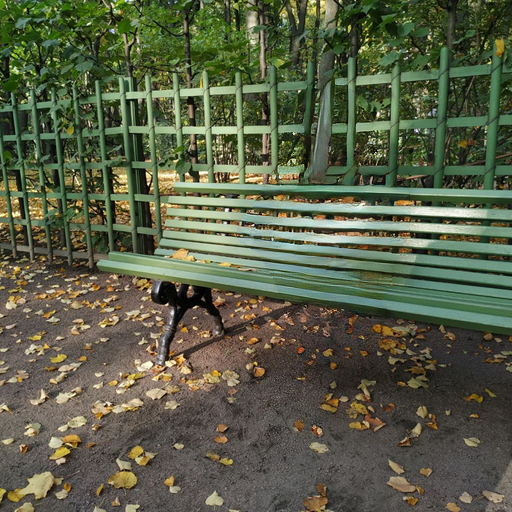
\includegraphics[width=.9\linewidth]{c:/msys64/home/xinbinjian.sh/.org.d/roam/img/扩散模型_diffusion_model/_20230112_192258bench2_inpainted.png}
\end{center}
\begin{center}
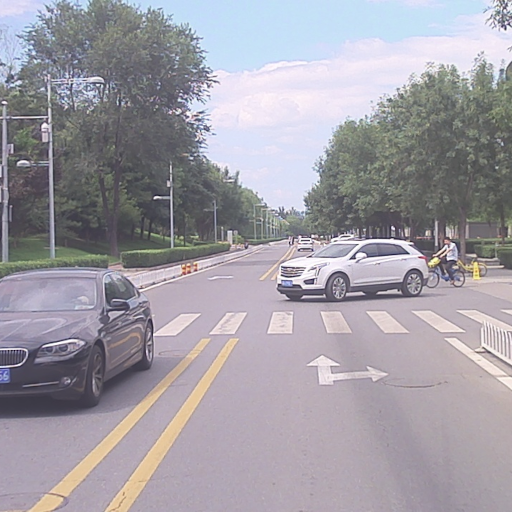
\includegraphics[width=.9\linewidth]{c:/msys64/home/xinbinjian.sh/.org.d/roam/img/扩散模型_diffusion_model/_20230112_1927141534313574.830631_crop.png}
\end{center}
\begin{center}
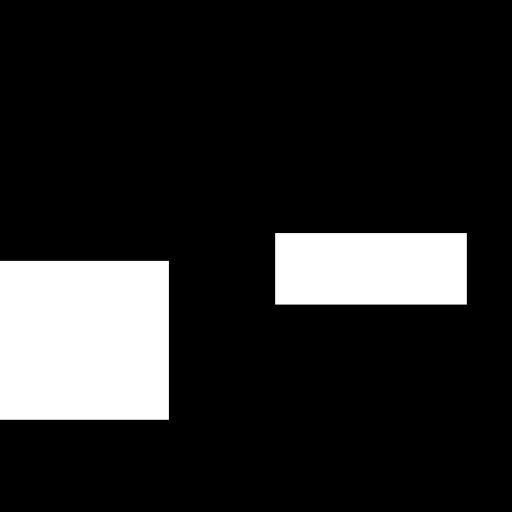
\includegraphics[width=.9\linewidth]{c:/msys64/home/xinbinjian.sh/.org.d/roam/img/扩散模型_diffusion_model/_20230112_1927211534313574.830631_crop_mask.png}
\end{center}
\begin{center}
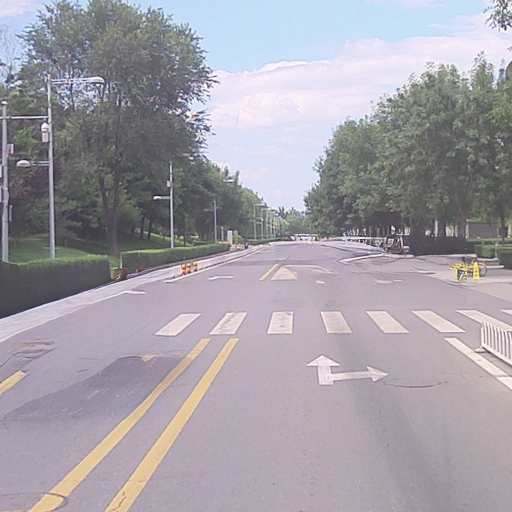
\includegraphics[width=.9\linewidth]{c:/msys64/home/xinbinjian.sh/.org.d/roam/img/扩散模型_diffusion_model/_20230112_1927311534313574.830631_crop_inpainted.png}
\end{center}
\end{document}
